\pdfoutput=1
\documentclass[onecolumn, draftclsnofoot,10pt, compsoc]{IEEEtran}
\usepackage{graphicx}
\usepackage{url}
\usepackage{setspace}
\usepackage[margin=0.75in]{geometry}
\setlength{\parindent}{0pt}
\usepackage[hidelinks]{hyperref}
\usepackage{courier}
\usepackage{listings}
\usepackage[final]{pdfpages}
\lstset{
    breaklines=true,
    basicstyle=\ttfamily
}
\usepackage{float}
 
\renewcommand\thesection{\Roman{section}}
\renewcommand\thesubsection{\Alph{subsection}}
\renewcommand\thesubsubsection{\arabic{subsubsection}}
\geometry{textheight=9.5in, textwidth=7in}
 
% 1. Fill in these details
\def \CapstoneTeamName{     Aerolyzer}
\def \CapstoneTeamNumber{       22}
\def \GroupMemberOne{           E. Reilly Collins}
\def \GroupMemberTwo{           Sophia Liu}
\def \GroupMemberThree{         Jesse Hanson}
\def \CapstoneProjectName{      Aerosol Analyzer Mobile Web Application}
\def \CapstoneSponsorCompany{   NASA JPL}
\def \CapstoneSponsorPerson{        Dr. Kim Whitehall}
 
% 2. Uncomment the appropriate line below so that the document type works
\def \DocType{      %Problem Statement
                %Requirements Document
                %Technology Review
                %Design Document
                Final Report
                }
            
\newcommand{\NameSigPair}[1]{\par
\makebox[2.75in][r]{#1} \hfil   \makebox[3.25in]{\makebox[2.25in]{\hrulefill} \hfill        \makebox[.75in]{\hrulefill}}
\par\vspace{-12pt} \textit{\tiny\noindent
\makebox[2.75in]{} \hfil        \makebox[3.25in]{\makebox[2.25in][r]{Signature} \hfill  \makebox[.75in][r]{Date}}}}
% 3. If the document is to be signed, comment the RENEWcommand below
%\renewcommand{\NameSigPair}[1]{#1}
 
%%%%%%%%%%%%%%%%%%%%%%%%%%%%%%%%%%%%%%%
\begin{document}
\begin{titlepage}
    \pagenumbering{gobble}
    \begin{singlespace}
        %\includegraphics[height=4cm]{coe_v_spot1}
        \hfill 
        % 4. If you have a logo, use this includegraphics command to put it on the coversheet.
        %\includegraphics[height=4cm]{CompanyLogo}   
        \par\vspace{.2in}
        \centering
        \scshape{
            \huge CS Capstone \DocType \par
            {\large\today}\par
            \vspace{.5in}
            \textbf{\Huge\CapstoneProjectName}\par
            \vfill
            {\large Prepared for}\par
            \Huge \CapstoneSponsorCompany\par
            \vspace{5pt}
            {\Large\NameSigPair{\CapstoneSponsorPerson}\par}
            {\large Prepared by }\par
            Group\CapstoneTeamNumber\par
            % 5. comment out the line below this one if you do not wish to name your team
            \CapstoneTeamName\par 
            \vspace{5pt}
            {\Large
                \NameSigPair{\GroupMemberOne}\par
                \NameSigPair{\GroupMemberTwo}\par
                \NameSigPair{\GroupMemberThree}\par
            }
            \vspace{18pt}
        }
        \begin{abstract}
        % 6. Fill in your abstract   
        \noindent Over the past few months, the Aerolyzer team has worked with our client to make progress towards our finished software product. The purpose of this document is to illustrate that progress and provide a retrospective of our work done so far. An introduction of our project, a discussion of changes to our requirements, design, and tech review documents, and introspective of our learning throughout the project are included. Additionally, this document contains our weekly blog posts, final poster, and project documentation. After demonstrating our aerosol-analyzing mobile application at Expo, this document serves as a thorough overview of our Aerolyzer project.
 
        \medskip
 
        In summary, we have completed several documents that aided us in figuring out how our project will come together and made changes to these along the way. Furthermore, we worked on several tasks assigned by our client and added these to our code repository comprising of our final product.  Lastly, we have continued making progress this term towards a better understanding of software design, the development process, and programming collaboration.
        \end{abstract}     
    \end{singlespace}
\end{titlepage}
 
%s\newpage
\pagenumbering{arabic}
\tableofcontents
% 7. uncomment this (if applicable). Consider adding a page break.
\clearpage
 
\listoftables
\listoffigures
\clearpage
 
\begin{flushleft}
% 8. now you write!
\section{Introduction}
Aerolyzer is a project that was requested by client Dr. Kim Whitehall in collaboration with Dr. Lewis McGibbney. She requested this project to develop an application that supports the ability to understand content from images, and encourage human curiosity in nature. The development of this application is important because provides citizen scientists with the ability to understand the aerosol content of their image, as well as provides scientists with a large database of aerosol data throughout the globe. The members of our team consist of Oregon State University students Reilly Collins, Sophia Liu, and Jesse Hanson, as well as clients Dr. Kim Whitehall and Dr. Lewis McGibbney. As for the students' individual roles, Reilly and Sophia focused mainly on frontend and database development, while Jesse focused on developing the backend image processing. The role of clients Dr. Kim Whitehall and Dr. Lewis McGibbney was mainly to supervise and facilitate our progress, although Dr. Kim Whitehall also contributed to the development of our project.

\section{Requirements}
\subsection{Original Requirements Document}
\clearpage
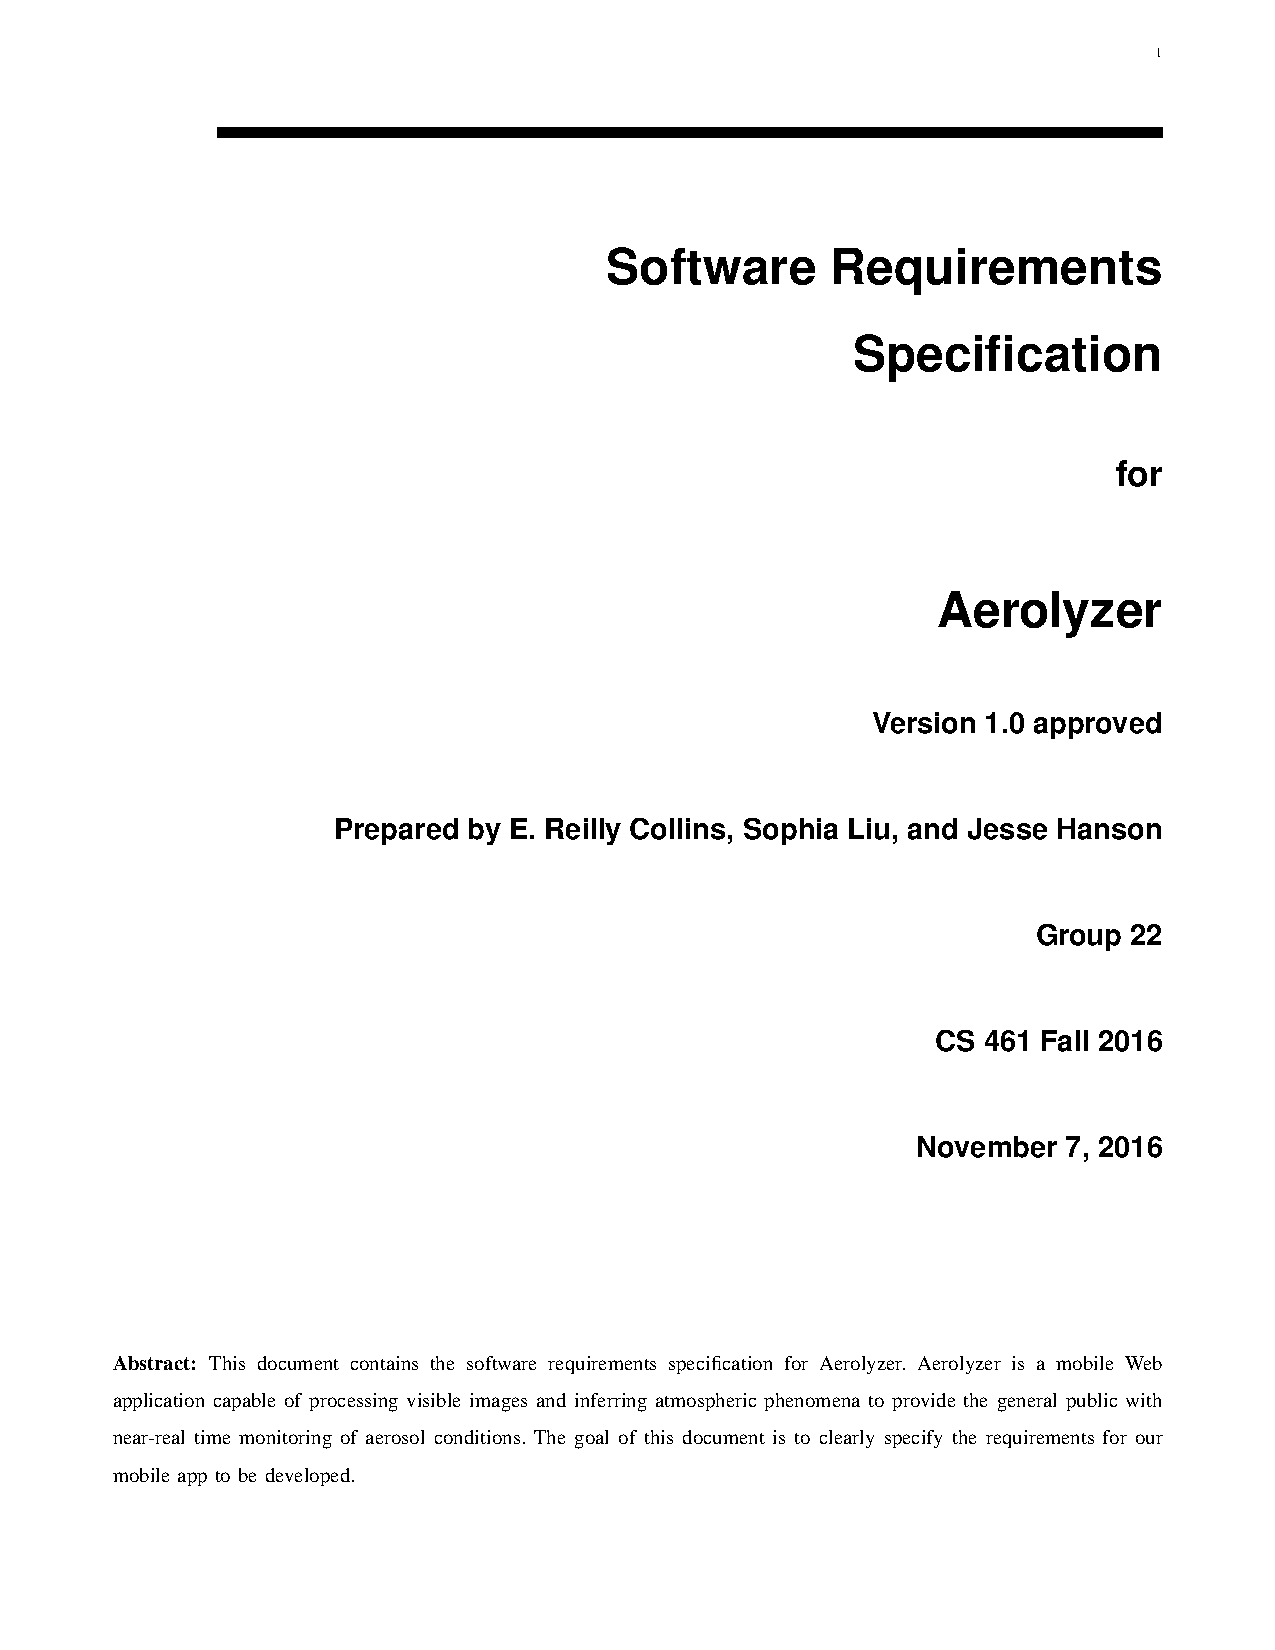
\includepdf[pages=-]{Aerolyzer_Requirements_Original.pdf}
 
\subsection{Original Gantt Chart}
\begin{figure}[H]
\centering
  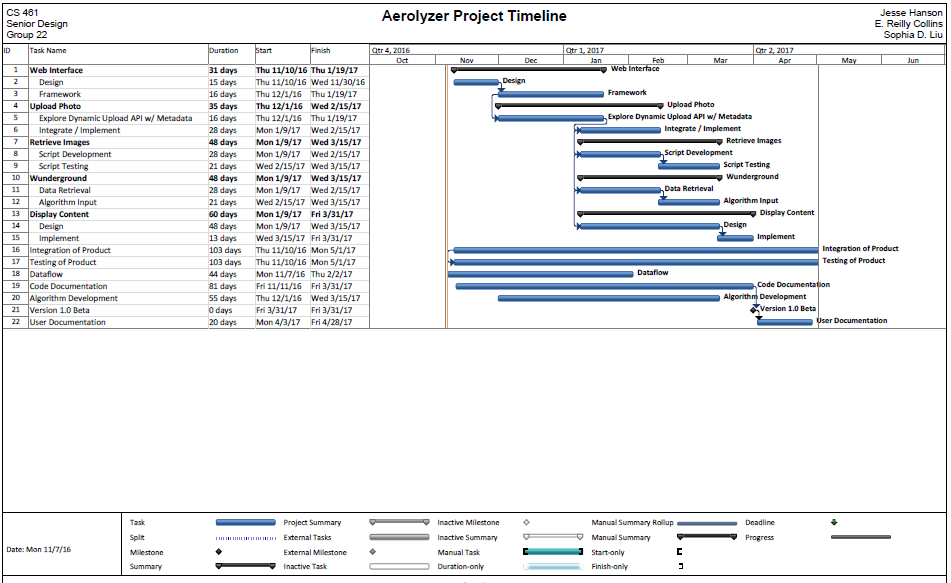
\includegraphics[width=\textwidth]{gantt_original.PNG}
  \caption{Original Gantt chart for requirements}
  \label{fig:gantt_original}
\end{figure}
 
\subsection{Client Requirements Document Changes}
The basic functionality of our product outlined in our original requirements document remains unchanged. However, one major aspect of our project that differs from the description in this document involved the actual core color-analyzing aerosol algorithm. Our client relayed to us that she overestimated our time commitment to the project, as well as the freedoms for her to guide the project as the client. Instead of working on both computer science and atmospheric science aspects of our development, we chose to focus only on the computer science component. This change means our final product only met requirements 1-5 (rather than all 7), and "Display of Aerosol Content" requirement 3 does not actually display output from the core algorithm yet. The atmospheric science component will be completed by a capstone team next year. 
 
Our "Extract EXIF Information From Data" requirement 4 also changed, essentially being split up into two different EXIF-related requirements. A script was written that scrapes the category and tags from online images as a list, then outputs this data into a JSON file to be stored on Github and used to improve the color-analyzing algorithm. Our webapp itself also has a script that retrieves EXIF data from uploaded photos and returns required EXIF data as a dictionary to be used in the core algorithm; all photos and EXIF data are stored in our image repository as described in the requirement. 
 
Other (mostly minor) changes to requirements are listed as comments in table \ref{table:1}.
 
\begin{table}[H]
\caption{Functional requirement changes}\label{table:1}
\centering
\begin{tabular}{| p{1cm} | p{5cm} | p{5cm} | p{4cm} |}
\hline
\textbf{Num} & \textbf{Requirement name} & \textbf{What happened} & \textbf{Comments}\\
\hline
1 & Web Application Interface & Removed mobile-only restriction; instead, users can access website via desktop and are simply notified if uploaded image does not meet mobile-only restriction. This change was made to reach a wider range of users after discussion with our client. & Functionally unchanged. \\
\hline
2 & Upload Photo & Minor text difference: "Use Photo" button changed to "Submit" button as a simple UI decision. & Functionally unchanged. \\
\hline
3 & Display of Aerosol Content & Actual aerosol content is not displayed due to core algorithm not being implemented until phase 2; however, the page is displayed as described and there is a blank box where aerosol content will eventually be shown. Minor text difference: "Cancel" button changed to "Upload" button cancelling current upload as simple UI decision. & Functionally unchanged. \\
\hline
4 & Extract EXIF Information From Data & Split into two EXIF-related requirements. This change was made as our client needed both test data to improve the core algorithm (e.g. verify the algorithm could correctly detect sunsets from an image with a "sunset" category) and actual EXIF data from an uploaded image to get that image's aerosol content. & Details explained wholly in above subsection introduction. \\
\hline
5 & Using Weather Underground API & & Functionally unchanged. \\
\hline
6 & Get Data From Satellite Source & Removed in phase 1 (development phase). Will be implemented in phase 2 (atmospheric science phase). & Details explained wholly in above subsection introduction. \\
\hline
7 & Running the Core Algorithm &  Removed in phase 1 (development phase). Will be implemented in phase 2 (atmospheric science phase). & Details explained wholly in above subsection introduction. \\
\hline
\end{tabular}
\end{table}
 
\subsection{Final Gantt Chart}
\begin{figure}[H]
\centering
  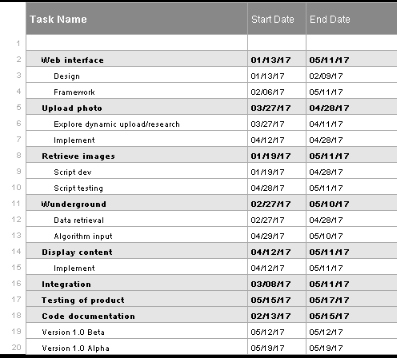
\includegraphics{gantt_final1.PNG}
  \caption{Final Gantt chart requirements}
  \label{fig:gantt_final}
\end{figure}
\begin{figure}[H]
\centering
    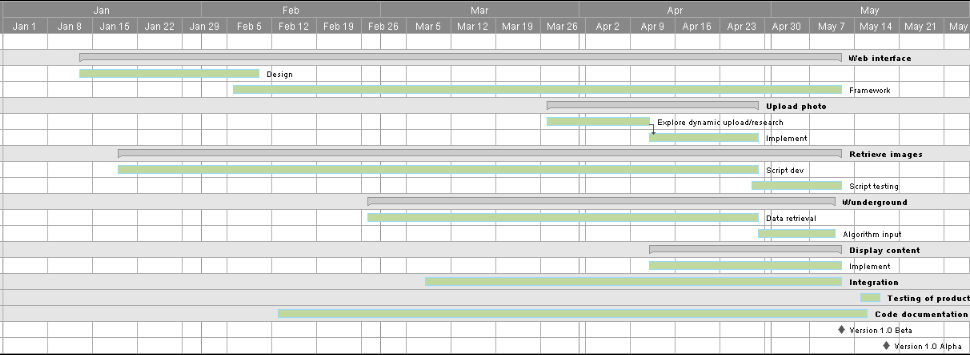
\includegraphics[width=\textwidth]{gantt_final2.PNG}
  \caption{Final Gantt chart timeline}
  \label{fig:gantt_final}
\end{figure}
 
\section{Design}
\subsection{Original Design Document}
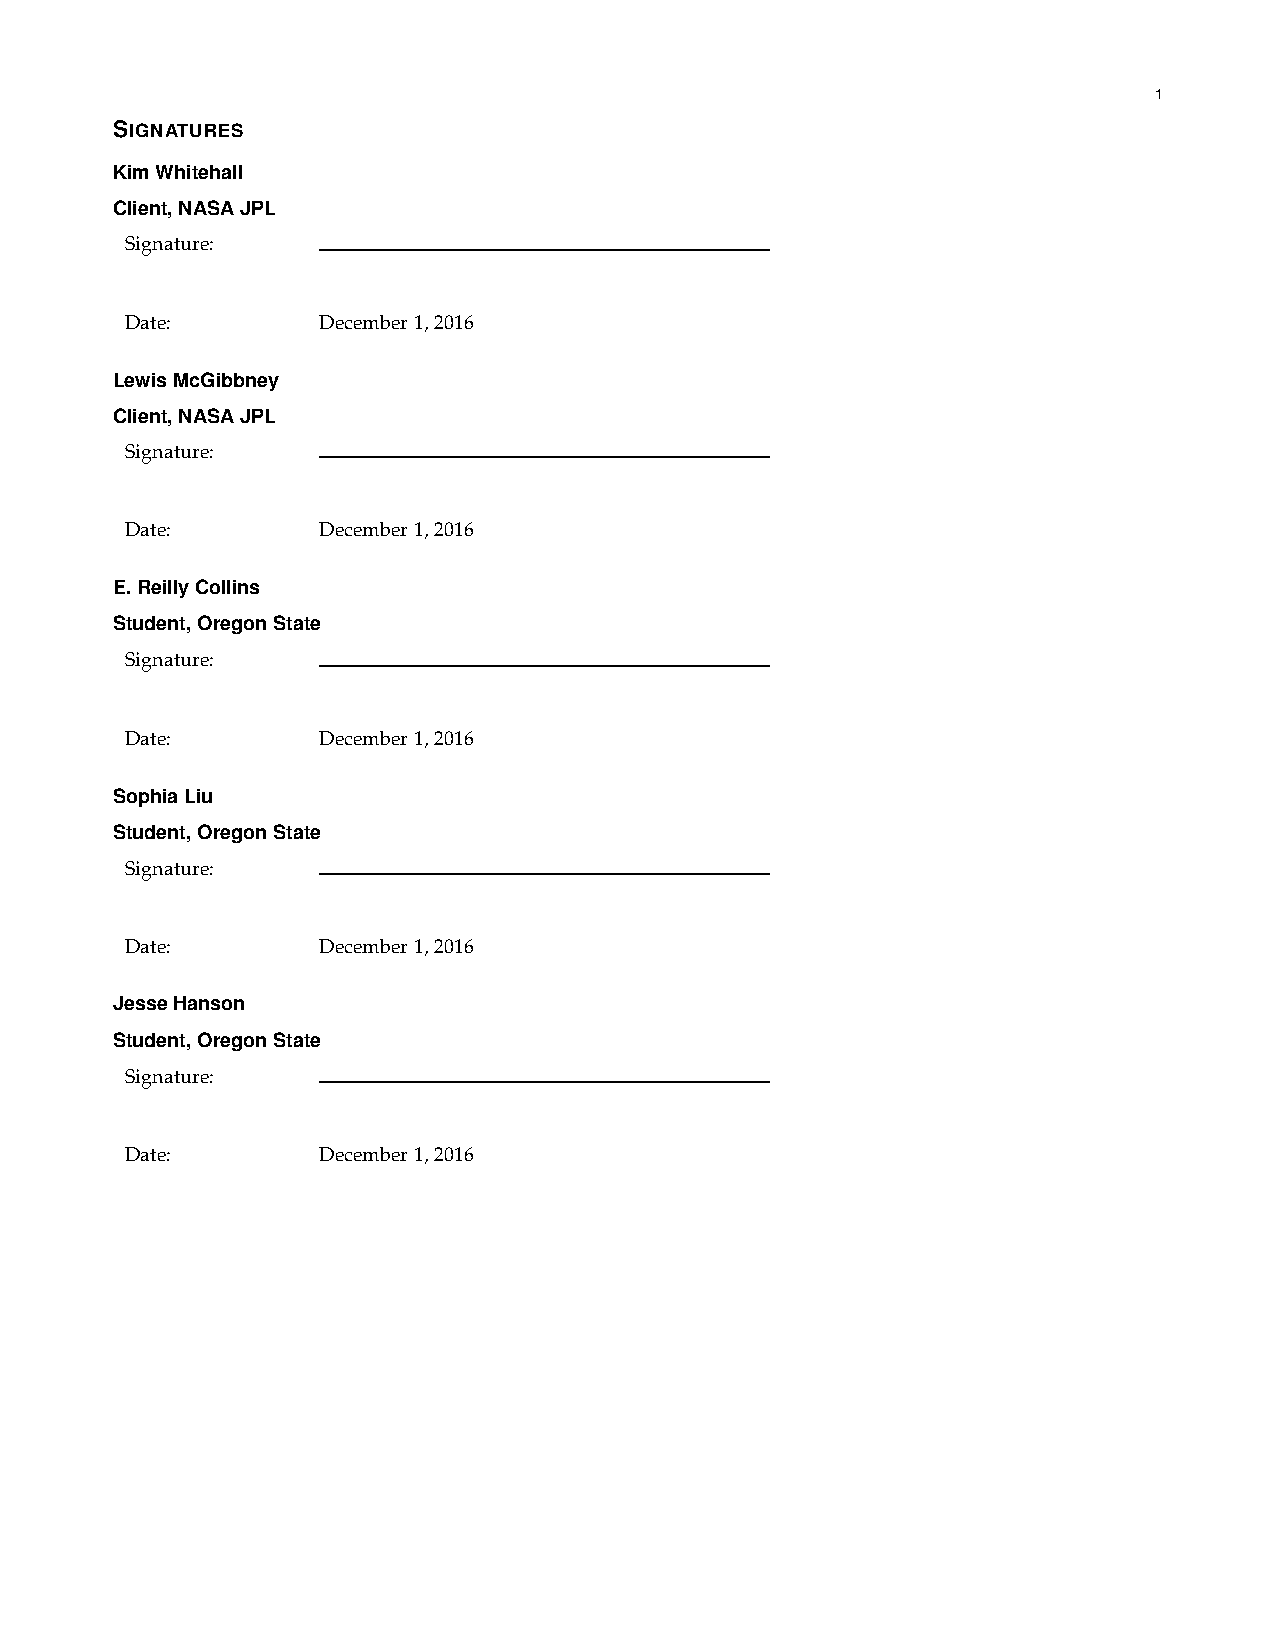
\includepdf[pages=-]{Aerolyzer_Design_Original.pdf}
 
\subsection{Design Document Changes} 
The design document did not have any large changes over the course of the year. The only change our team made was to change the database schema to have three tables instead of four tables. The original schema had a table for image data, acquired via EXIF metadata extraction; a table for geo-related data, acquired via MISR; a table for weather data, acquired from Weather Underground; and a table for the core algorithm's output, acquired after running the core algorithm successfully and receiving output. Our new schema has the images table, a table for image data acquired via EXIF metadata extraction, geo-related data acquired via MISR, weather data acquired from Weather Underground, the core algorithm's output acquired after running the core algorithm successfully and receiving output
 
\section{Tech Review}
\subsection{Original Tech Review}
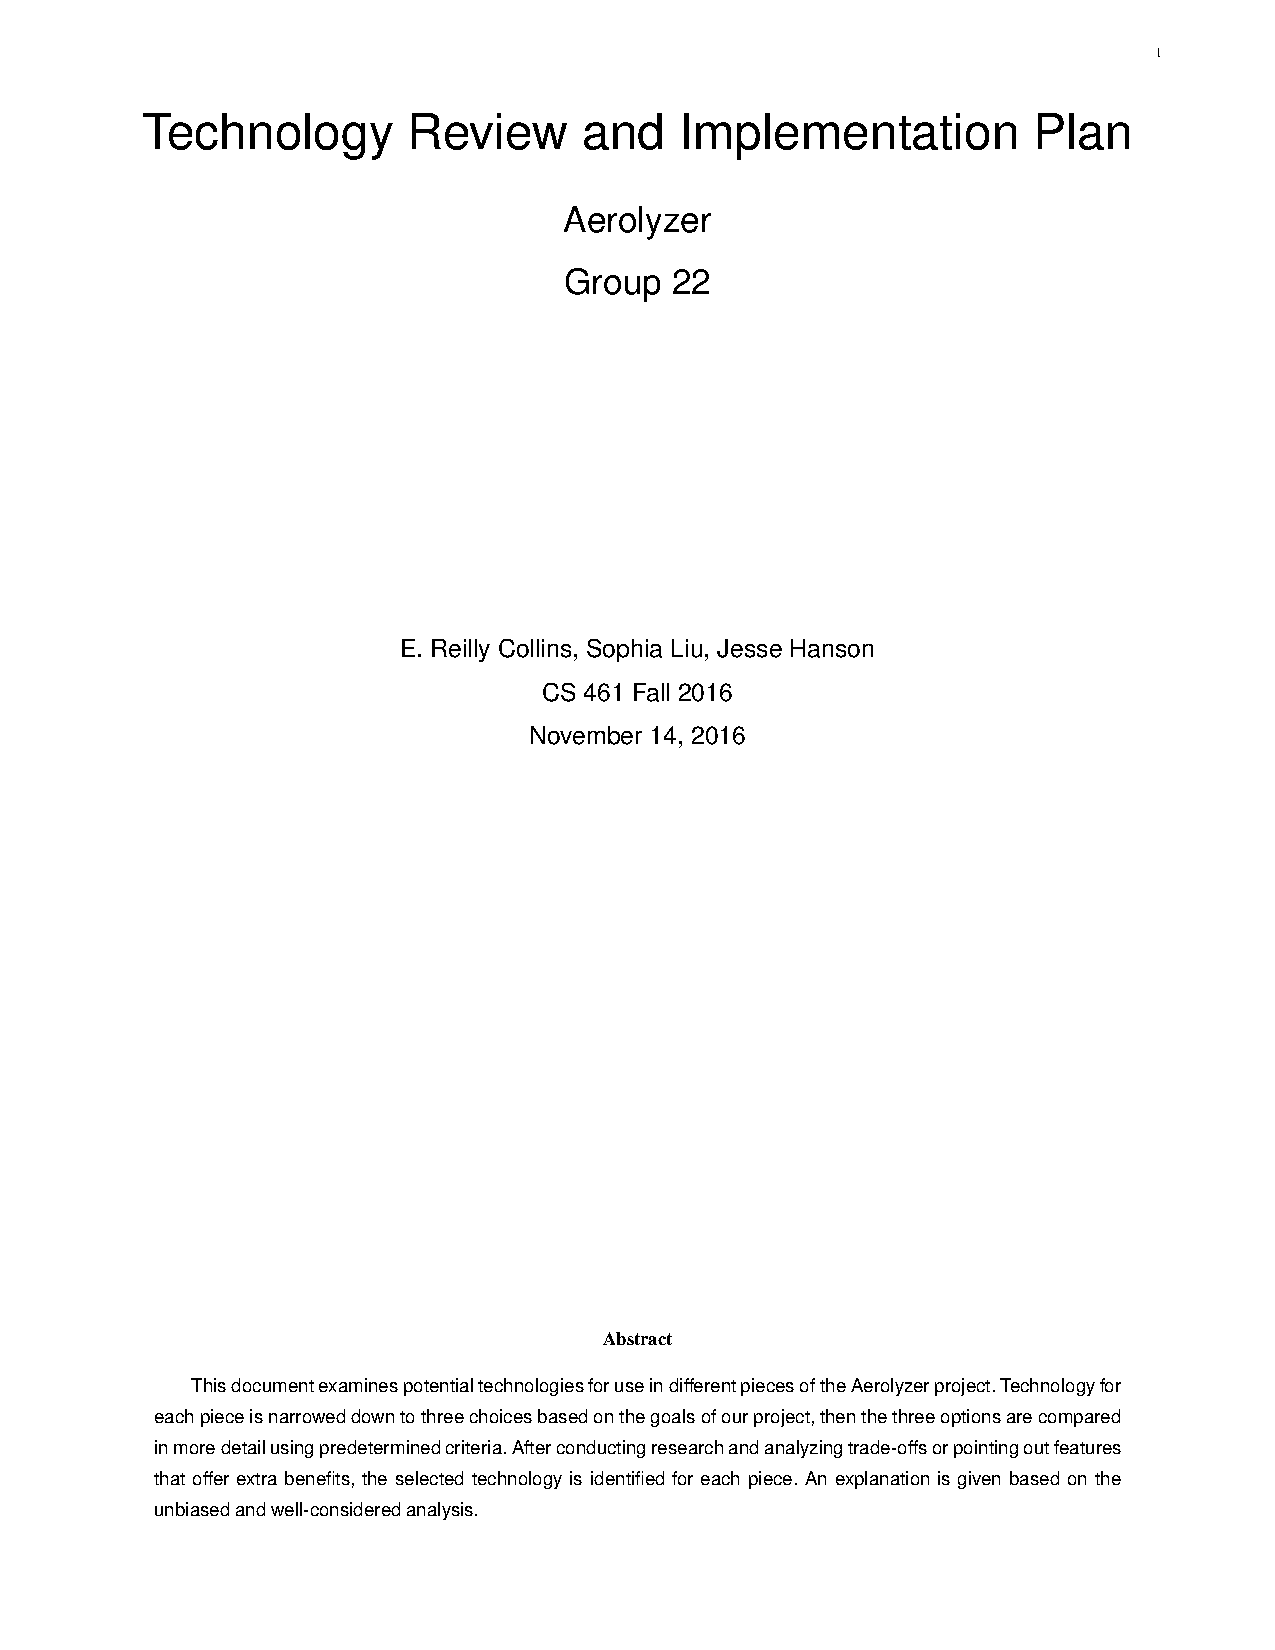
\includepdf[pages=-]{Aerolyzer_TechReview_Original.pdf}
 
\subsection{Tech Review Changes} 
We changed two technologies throughout the course of the year. One of these changes was to use Apache Solr instead of MySQL for our database. We decided to make this change after the scope of our project changed and Solr fit our database criteria better than MySQL did. Solr had much better scalability compared to MySQL. Solr is also completely open source and is part of the Apache brand. The other technology we changed was the use of DropzoneJS for uploading files. After beginning the web framework implementation with Django, we discovered that Django offers a simple file upload that would make it easier to add files directly to our app's file system. We also realized that we would probably not need to make use of DropzoneJS's drag-and-drop upload feature, as our main focus was creating a mobile webapp - mobile devices typically do not allow for drag-and-drop file system uploads.
 
 
\section{Weekly Blog Posts} 
\subsection{Fall Term}
\subsubsection{Week 1}
\paragraph{Reilly}
 
Next week, we will meet with Vee on Monday for the first time. Our expectations for the project right now are just to do some more research on atmospheric optics and image/feature detection. I will also do more research on UI for our app and check out some of similar apps that Kim shared with us.
 
Last Friday was our first meeting with our client, Kim Whitehall and Lewis McGibbney from NASA JPL. After our meeting, Kim sent us some resources via links to look through to help us get started - I looked through these and got a better understanding of our project, which was really helpful for working on the problem statement document. Based on my interest in UX, I was given the tentative team role of looking into the UX component of our app; I explored some options for us to display our photos, as well as how the app will look/feel, by researching other photo sharing and feature detection apps (both for Android and iOS).
 
Over this past week, we completed our problems statement assignment by creating the LaTeX file and Makefile to compile a PDF for Kim and Lewis. They gave us feedback on our draft and approved the final version, which was signed and sent back to us to turn in.
 
Our Github repo was also created this week; I pushed all of our problem statement files into a new directory.
 
 
As a group, we aren't sure whether we are able to make the Github repo public and use an organization or if we are restricted to just private repos. Kim and Lewis are going to contact the professors about this. Personally, I haven't encountered any problems this week.
 
\paragraph{Sophia}
 
This week, we will be continually doing research on our assigned topics. I am working on getting acquainted with Dust. We will be meeting with our TA on Monday to check in on our project progress.
 
 
On 10/14 we met with out client Kim Whitehall and Lewis McGibbney. On 10/9 Dr. Whitehall sent us numerous resources to research during the week. I did a lot of research on the Aerosol Content and Rust. This week we also wrote and all signed our problem statement. The problem statement summarized what us and our clients expectations were for this senior capstone project. All of the parties signed the statement. We also set up this github page and will started updating the WIKI page.
 
 
Our group and our clients have been working really well together. The only problem I have encountered so far is that the papers regarding the Aerosol content have been difficult to understand, but after some research I am confident that I will have a firm understanding on the topic. Another problem is having a private repo but having a public repository is causing some issue in Github.
 
\paragraph{Jesse}
 
For this week we will continue to conduct individual intensive research to gain background knowledge on the topics at hand. We will be meeting with our TA this Monday to analyze our progress.
 
 
We met with our client last week on Friday to determine what the goals of our project will be. We identified individual research agendas, and read articles that helped us to build knowledge on the subject at hand.
 
 
So far our group has worked well together, the only troubles we have encountered have been difficulty limiting our project to certain main goals, as well as researching articles on the topic at hand. Our weekly meetings have been well put together, but we hope to work on having productive conversations throughout the week as well.
 
\subsubsection{Week 2}
\paragraph{Reilly}
 
This upcoming week, our team plans on continuing research as documents come in from the group mailing list. We will also complete any outstanding tasks that Kim asks us to work on throughout the week, such as contributing more to our readme. We have revised our problem statement and will make further revisions using feedback from our professors, then send it to our clients for more feedback and signatures.
 
Our requirements document is due (signed) on Friday, so we will be working on that this week with our clients as well.
 
 
We met with our TA Vee this week and discussed what to anticipate for our project. He went over some of the expectations for the class and gave us advice on working as a team, interacting with our client, and completing work for the capstone class.
 
After meeting with Kim on Friday, I setup our updates wiki page and created links for our weekly updates. I have continued working on UX research, as well as reviewing various documents that Kim has been sending to our mailing list. Specifically, I looked at Android UX examples for taking and displaying photos; I also skimmed through the Android design guidelines to get a better feel for typical photo-centric app layouts and formatting.
 
 
We resolved an issue from last week by moving our repo under our new Aerolyzer organization and making it public. There are no other problems we've run into since last week.
 
\paragraph{Sophia}
 
This week I focused on reading through the provided research papers more. I have started going through the REST API's Documentation and been watching more tutorials.
 
 
This week I plan to do a mini project with REST, and continue to familiarize myself with the research papers. I want to have a solid understanding on the science behind our project by the end of the week. I also need to work on the requirement document and have it to our clients this week.
 
 
Our problem statement had to be redone, so we are working on it. We resolved the issue with the private vs. public github repositories. Our github repository is now public, and so are all of our profiles on it.
 
\paragraph{Jesse}
 
This past week our main focus was to conduct more research and further develop our knowledge on the topic of our project. I looked up professors at OSU with a background in optics, and found a professor within the physics department that I plan to meet with to discuss ideas for our project. This week was extremely busy for me, so I did not have as much time to read articles and other papers as I did last week. However, I downloaded iPython which will allow me to play around with MatPlotLib this upcoming week.
 
 
This week I plan to become familiar with MatPlotLib, as well as identify some sunset images that we can begin to look at for our project. I also look forward to reading more documents which have been provided by our client. Our team will also be focused on revising our Problem Statement and developing our Requirements Document which are currently due 10/26/16 and 10/28/16 respectively.
 
 
One issue we had was satisfying our client's desire for a public github repo, as opposed to having a private repo which our professor specifically asked for. However, we were able to remedy this with permission from our professor to create a public repo that satisfies both parties needs. Technically speaking, another problem we encountered was having to revise our Problem Statement.
 
\subsubsection{Week 3}
\paragraph{Reilly}
 
This upcoming week, our team is going to complete the requirements document and have it signed by the client. We will have to complete this by Friday. The team is planning on going over the specifics of our requirements doc on Monday during our meeting with our TA.
 
My other plans for this week are to continue looking at research documents sent by our client, as well as review the github workflow doc.
 
 
This week, the team and I updated our problem statement using feedback from our professors, as well as suggestions from our client. We definitely have a much better understanding of our project now; everyone on the team is on the same page. A final hard copy was turned in, and I committed the final unsigned version on our repo.
 
We also got started on our requirements document this week. This was challenging at first, but ultimately it's been helpful to figure out what exactly we are going to be doing for the rest of our project. Going through requirements during our meeting with Kim on Friday was helpful for completing the doc as well.
 
 
We have not encountered any major problems this week. At first, we weren't sure where to get started with our requirements doc, but after looking through examples and meeting with our clients we have a solid understanding. Our requirements doc is well underway, with a draft complete and final (signed) version on track to be finished by the Friday due date.
 
\paragraph{Sophia}
 
This past week we again focused on reading the research papers provided by our client. I added a description to the Github page, and we finished and signed the problem statement.
 
 
This upcoming week were are going to ad coding task. We are also continuing to read research papers, and finish editing and adding to our requirements document.
 
 
Our problem statement was returned to us, and we edited and updated it.
 
\paragraph{Jesse}
 
This past week we again focused on researching while also accomplishing a few tasks. I read a couple of papers supplied by our client, as well as added the Apache License v2.0 to our source code in GitHub.
 
 
This upcoming week were are going to play around with some code focused on gathering landscape and sunset images from a website. We are also continuing our research while wrapping up our requirements document.
 
 
We didn't encounter any significant problems this past week.
 
\subsubsection{Week 4}
\paragraph{Reilly}
 
This upcoming week, I am going to work on the second coding task given to us by our client. This task involves creating a script in Python that will scrape images and metadata from Weather Underground, and we will eventually use these images in our color-analyzing algorithm.
 
I will also work on our technical review document this week, as it is due Friday, though the assignment itself hasn't been released yet.
 
 
This week, we finished our requirements document as a team. There are some sections that we couldn't fully complete, as they depend on completing further research regarding the color-analyzing aerosol algorithm, but we just made note of that in the document and will add to it as needed. During our meeting on Friday, Kim and Lewis helped us walk through the requirements to make sure everyone was on the same page. It sounds like our clients are very happy with our requirements and can see the project coming together. We have a pretty good understanding of what we need to accomplish in the coming months and what we still need to find out through exploration and discussion.
 
I also worked on our first coding task this week. This task involved writing a Python program that used the Weather Underground API to retrieve data about given cities around the world. We were assigned this coding task as practice for retrieving meteorological data needed for the color-analyzing aerosol algorithm. The Wunderground API seems pretty useful for our needs, especially considering it's the free version.
 
 
I had some questions about our problem statement feedback, so I talked with Kirsten this week to better clarify what problem we are trying to solve with Aerolyzer. She helped me work through finding the best way to convey our project's goal to others and helped me understand how we could make our web app marketable.
 
Our team had some problems working on the Gantt chart, as we weren't given any direction on where to start in class. Kim and Lewis helped us write out tasks to be completed until Expo based on our functional requirements, and we converted those into a working Gantt chart.
 
\paragraph{Sophia}
 
This week I will start working second coding task given to us by our client. It is a script to provide a multipanel look at the color channels in a given image. I will also work on our technical review document this week, as it is due Friday.
 
 
This week, we finished our requirements document. There are some use cases and requirements we will continue to add as needed while we finish the planning stage of our application. We all agree that it is very exciting to see our project form from ideas, to an actual application.
 
 
We had some issues with creating the Gantt chart. With some help from Dr. Whitehall we planned it during our meeting on Friday and we implemented it.
 
\paragraph{Jesse}
 
For this week, we spent the majority of our time finishing up our requirements document. The Gantt chart took us quite a bit of time to complete, mainly because we were unsure how to create one. However, we got help from our client during our weekly meeting and were able to complete it based on that information.
 
 
Our problems for this week came from difficulties in creating the Gantt chart. However, as I mentioned we were able to figure it out by communicating with our client.
 
 
This upcoming week we have a few tasks to complete. We need to begin working on our tech document, as well as work on a few of the coding tasks that have been assigned to us by our client.
 
\subsubsection{Week 5}
\paragraph{Reilly}
 
This upcoming week, our team is going to turn in the tech review document. We are also going to work on implementing some of the discussed technologies in our Tech Review. My job will be to implement Pylint for use in our coding environment - to do this, I will setup a configuration file and add a supporting wiki for documentation. I have already done research on Pylint for our tech review, so I should be able to quickly add the config file and wiki.
 
The team is going to discuss these added technologies during our meeting on Friday.
 
 
This week, we turned in our requirements document and started the tech review doc. We met with our client on Wednesday to discuss the technologies we would be using, and we came up with 9 different pieces of the Aerolyzer application that we could research to find alternative technologies. My three sections of the requirements doc are the coding environment, image and metadata storage, and extracting EXIF metadata.
 
I also created an issue for, committed, and submitted a pull request for our final (unsigned) requirements files on our repo.
 
Finally, we received feedback about our requirements document on Friday. We will need to make the suggested changes to our doc for the final document before we put everything together at the end of the year. We will also apply the general critiques to our documents going forward (e.g. formatting).
 
 
Our client gave us several suggestions for improvement on our requirements document and Gantt chart the day that it was due, so we spoke with our TA and were able to turn it in a day later than discussed.
 
Since we had already decided on a few of the technologies we would be using as a team, our client asked the professor about what was required of the tech review assignment. She didn't think we should spend time searching for alternatives when we had already decided to use and begun moving forward with specific technologies. She told us that he said we only had to compare technologies where possible, meaning we did not have to research alternatives for technologies we had already selected.
 
\paragraph{Sophia}
 
This upcoming week, we are working on and turning in the tech review document. We are also going to work on implementing some of of the technologies into our github repo. Specifically for me I am working on integrating Travis CI and Coveralls support.
 
 
We complete and submitted our requirements document and started working on the tech review doc. We met with our Dr. Whitehall on Wednesday to discuss the tech review document, and what technologies we would be using for it. We came up with 9 section of the Aerolyzer application to research alternate technologies, and we each are in charge of 3 sections. My three sections are the web interface, testing, and getting meteorological data.
 
 
We received feedback on our requirements document and had some minor issues, so we will be working on fixing the requirements document based on what our TA said. We also had some issues getting our Gantt Chart and requirements done on time, so we received an extension on it.
 
\paragraph{Jesse}
 
We made quite a bit of progress this week, finishing up our requirements document and beginning our tech document. Since there was no school Friday, we met with our client on Wednesday and went over how we are going to complete our tech document. I was assigned sections including Upload Photos, Getting Geo-related Data, and Documentation/Development of API Documents. I also looked into one of our coding assignments from our client, and look forward to working on it further.
 
 
We had no major problems, however our client wanted to email our professor about the necessity of the tech document. She was concerned because we already have most of our technologies figured out, so she wanted to make sure we weren't doing unnecessary work.
 
 
For this upcoming week, we will finish up our tech document and turn that in. We also have individual coding assignments that we will be working on throughout the week.
 
\subsubsection{Week 6}
\paragraph{Reilly}
 
This upcoming week, our team is going to begin working on our design doc. We will look into the IEEE Std 1016-2009 document and research examples to get started with our design. We will also talk to our client about the design doc as we work on it (via slack) in order to clarify anything we aren't sure about. Finally, we will need to discuss which parts of the design doc each of us will work on in addition to writing about our specific technologies from the tech review. The design is our only class assignment to work on this week.
 
During our meeting Friday, we went over some of the code guidelines that should be implemented in the Pylint file. I am going to continue working with the team to come up with a style for Aerolyzer. Should they change as time goes on, I will add these configurations to the aerolyzer\_lint\_file in the repo.
 
 
On Monday, I turned in our tech review files via github. For the tech review, I researched technologies for our coding environment, database, and EXIF metadata extraction. Our team had already chosen to go with Pylint for the coding environment, so I talked about moving forward with that in the tech review. Then, after completing research and analyzing tradeoffs, I concluded that we would use MySQL for a database and the ExifRead Python package for extracting EXIF data. I also started our design doc by creating a tex template, along with other needed files (such as a Makefile, IEEE files, and a bib file). We aren't yet sure what sections will be required for the design, so at the moment our template has the same sections as the IEEE Std document. We will change these once we get a chance to discuss the exact format with our TA and/or professors.
 
Lastly, I committed a Pylint file for our project called aerolyzer\_lint\_file in the repo. I will be in charge of maintaining this file going forward. I also added our Pylint information to the wiki. Our TA told me I could install files on the school server without root privileges using the command "python setup.py install --user," and this allowed me to get Pylint setup in my own coding environment.
 
 
I ran into a problem checking in our tech review files: somehow I was unable to push changes to my specific branch for the tech review issue I created. I ended up adding files manually via the online github interface in order to meet the midnight deadline. Over the next few days I tried to figure out what went wrong, but I'm still not sure; I was able to get back on master and then on a new branch to check in my pylint files with no issues. The problem seems to be fixed, though, so hopefully I don't run into this issue again.
 
\paragraph{Sophia}
 
This week, our team will begin working on the design doc. Since our client will be out of town for the next few weeks, we will be communicating via slack. I will also work on adding more content to the .travis.yml file I added to the code base last week.
 
 
We turned in the tech doc on Monday. I was in charge of 3 sections, and finished my research and we turned in the document on time. I also worked on implementing TravisCI and Coveralls to our code base. This took awhile because I have never used TravisCI or Coveralls before, so I had to do some research to figure out how to implement them.
 
 
I ran into the problem of implementing my .travis.yml file to integrate TravisCI to our code base. I was confused about what to add to the content of it, but Lewis was really helpful during our team meeting and gave me an example of what to add to it. I also ran into the issue of adding Coveralls to the main repo, and not just my personal repo. I learned that I have to go into the settings for the main repo and change the settings to allow coveralls to be implemented to it.
 
\paragraph{Jesse}
 
This week we finished up our tech document and submitted it to github. We each completed 3 of 9 sections for the tech document, and after doing some research on certain technologies we were able to figure out what tools we will be using for our project. I looked into a personal assignment given to me by our client which requires me to create a skeleton for Sphinx documentation.
 
 
Overall we did not really encounter any problems this week. We had a few issues committing our changes to our repository, however I believe we figured them out (I was not the one trying to commit but I see the changes so I assume they were fixed). I was also slightly concerned that our tech document may have not been received due to these issues, but hopefully that is not the case.
 
 
For this upcoming week, we will not be meeting as a group due to the Thanksgiving holiday. However, we will be communicating through email and Slack. I will also be working on creating the actual skeleton for the Sphinx documentation, as well as offering help to Sophia on getting our framework setup in github.
 
\subsubsection{Week 7}
\paragraph{Reilly}
 
This week, I am going to continue working on the design document and the progress report. We will (hopefully) have the design document finished by Wednesday, then receive feedback and make changes before getting signatures and turning in a hard copy on Friday morning. Throughout the week I will also continue adding to the progress report based on how we decide to divide up the work as a team. We will not have a meeting this Friday due to our client being on vacation.
 
 
This past week, I have worked on the design document and completed close to half of it. I added a tex template with filled in sections to our github repo. I also started a document for our progress report. Finally, my pylint code pull request was approved and merged.
 
 
We are confused about our feedback on the tech review. Our client told us that one of our professors said we did not have to compare different technologies for pieces of the system that we had already moved forward with implementing, as that would be an inefficient use of our time. However, a different professor graded our assignment, so we believe there was a miscommunication and we received a poorer grade as a result.
 
\paragraph{Sophia}
 
This week, I will work both the design document and the progress report. We will try to finish everything by Wednesday to send to our clients for feedback. I will also work on fixing the TravisCI yml file by changing the content based on feedback from our client.
 
 
This past week, I worked on integrating travisCI with our code base.
 
 
I implemented the travisCI yml file, but there was still some issues with the content so I need to go back and fix/add some things to it. I also was confused about the feedback on the tech review, so I will go in and talk to our professors about it.
 
\paragraph{Jesse}
 
This week, we mainly worked on developing the design document and looked towards the final progress report. Since we need to run our design document by our client for approval, our plan is to complete the document by this upcoming Wednesday.
 
 
This week we did not really encounter any problems. Aside from issues in the grading on our tech review, and not knowing our score for the requirements doc, we did not have any issues.
 
 
For the upcoming week, we plan to finish our design document which is due Friday, and start on our progress report. Our goal is to complete the design document by this upcoming Wednesday so that we may get approval by our client before the submission deadline.
 
\subsection{Winter Term}
\subsubsection{Week 1}
\paragraph{Reilly}
 
This week, we met with our client and discussed our plan for the upcoming term. Using our Gantt chart from last term as a guide, the team will begin image scraping and designing our web interface this week. Though we will work together to accomplish these tasks, I will specifically focus on image scraping while Sophia and Jesse will focus on the wireframe prototype for our app.
 
 
Over winter break, I updated our tech review and design to reflect our choice of Apache Solr for our data storage rather than MySQL. Our client mentioned that scalability will be our most important database criteria, and adding this criteria revealed that Solr would be a better option than MySQL or MongoDB. We will therefore implement our database with Solr going forward.
 
 
We did not encounter any problems this week.
 
\paragraph{Sophia}
 
We are following the out Gantt chart so we will be starting to work on the web interface this week. Jesse and I will focus on making a wireframe prototype using Balsamiq. Reilly will work on image scraping Weather Underground.
 
 
We did not encounter any problems this week.
 
\paragraph{Jesse}
 
After meeting with our client, my plans for the coming week are to work with Sophia to create a wireframe of our website.
 
 
Since the past week was Winter Break, I did not really make any progress since last week.
 
 
I did not encounter any problems.
 
\subsubsection{Week 2}
\paragraph{Reilly}
 
This week, we will be updating the wireframe prototype and figuring out which Bootstrap theme we will be using. Our client suggested some changes for the website design; we will implement these in our wireframe and complete this task by our meeting next Friday.
 
 
I pushed our updated Tech Review and Design to the repo. I also pushed the script for image scraping along with the image metadata as JSON files to the repo, then submitted a pull request.
 
The images themselves are in our shared Google Drive - our client will use these images for initial testing. The Python script uses the Beautiful Soup Python library to scrape the Weather Underground image gallery for pictures. Included in the retrieved data is the date taken, image filename, image URL, comma-separated categories for the image given by Weather Underground, and URL for the gallery page. This metadata is stored in a list of namedtuples and converted to JSON before being written to an output file. All images are then downloaded to the current directory. A command-line argument can be given to change the Weather Underground gallery page used to retrieve images.
 
 
Our client mentioned that uploaded images will need size and resolution restrictions. We will need to add these requirements to our Requirements doc at some point.
 
\paragraph{Sophia}
 
This week we will be taking feedback from our client and working on changing the wireframe prototype and figuring out which Bootstrap theme to use.
 
 
I updated our travisCI.yml file. There are still some things I need to add. I also helped design our wireframe prototype. Some changes are still needed before our final wireframe is done.
 
 
Our client noted a lot of changes in our wireframes, so we will need to change some things. She also told me to add some things to the travisCI file which I am still a little confused about, so I will need to research more into it.
 
\paragraph{Jesse}
 
For this upcoming week, my plans are to update the wireframes so that they are much lower-level and similar to that of a prototype, as requested by our client.
 
 
This past week, Sophia and I used Balsamiq Mockups to create wireframes for our website. We tried to keep it at a high level and not get bogged down in the details.
 
 
One problem I encountered this week was miscommunication between our client and Sophia and I. Sophia and I both assumed wireframes to be more high level, while our client was expecting the wireframes to be more in-depth and similar to a prototype.
 
\subsubsection{Week 3}
\paragraph{Reilly}
 
This week, we are going to narrow down a specific Bootstrap theme and create our site's Home and About pages. This will give us CSS and a general skeleton to work with for implementing the rest of the site.
 
We will also be gathering EXIF data from various mobile images and aggregating info about mobile-specific tags. We will use the results to refine our restrictions, specifically the requirements that the image be taken on a mobile phone, free of editing/filtering, of type .jpg, and greater than a minimum resolution. We will be using Apache Zeppelin to accomplish this.
 
Finally, we will be looking into Exif.js as a way to import EXIF data from user's images in Python/javascript.
 
 
This past week, we worked on updating the wireframe prototype and created a working wireframe to guide our implementation. We also talked about the database design and came up with the tables for our schema. Our team is on the same page for our data flow, our UX, and how we will get data from users to our server.
 
 
Since we worked on our database design and made some changes, these will eventually need to be added to our Design doc. Additionally, we will probably end up using Exif.js for our implementation (rather than the ExifRead Python library); this change will need to be reflected in our Tech Review and Design doc as well. Finally, we will need to update our requirements to include a constraint for uploading only .jpg images.
 
\paragraph{Sophia}
 
This week we will continue on working on the wire frame using Balsamiq. We will work on refining the UX/UI to make sure our users have no confusion while using our application. We will also pick a Bootstrap theme to use throughout our web application. This will give us a skeleton to create our application on.
 
We will also be gathering and analyzing EXIF data extracted from various images taken on various mobile phones. We will be using this information to finalize our restrictions we will place on the images users can upload. We will specifically be using this to refine the size of the image we allow users to upload, but will also gather other useful data.
 
 
This past week we worked on creating a wireframe using Balsamiq. We also designed and made a UML diagram that represented our database schema.
 
 
We had some corrections to make to our UML diagram after meeting with our client.
 
\paragraph{Jesse}
 
For this upcoming week, my plans are to look into Python's exifread, and see how the EXIF data of a mobile image can be extracted.
 
 
This past week, we updated and completed the Balsamiq mockups for our website, which are now much lower-level and similar to that of a prototype.
 
 
I did not encounter any problems this week.
 
 
\subsubsection{Week 4}
\paragraph{Reilly}
 
This week, we will be working on implementing a Django framework for the frontend of our website and figuring out how to integrate our current HTML/Bootstrap CSS within that framework. I will also push our current HTML/CSS for our home page mockup to the Aerolyzer\_Website repo.
 
 
Last week, we picked a Bootstrap theme and created our site's home page. We also gathered EXIF data from various mobile images and aggregated info about mobile-specific tags. Those results enabled us to refine our restrictions, and we now specific EXIF tags/other values to check for when creating our script to verify user images.
 
 
We ran into some issues trying to setup a Django framework with the Bootstrap HTML/CSS that we already implemented. We will have to work through some tutorials or use other resources this week in order to get that set up.
 
Also, we will need to update our Requirements to reflect our updated restrictions for uploading a photo. We now have determined 8 different requirements that need to be met in order for our color-analyzing algorithm to work correctly.
 
Finally, we decided to use ExifTool instead of ExifRead to gather EXIF metadata and will need to update our Tech Review accordingly.
 
\paragraph{Sophia}
 
This week we will be working on downloading and going through the Django tutorial. Jesse and I will also start writing the pseudo code for the restrictions for the user to upload images.
 
 
Last week we picked a Bootstrap theme for our web application. We also gathered EXIF data from various mobile images using ExifTool. Reilly uploaded the images to Zeppelin because both Jesse and I could not get Zeppelin to download properly on our computers. We now have the information we need to finalize the restrictions we will place on the images to upload.
 
 
I could not get Zeppelin to download properly on my computer. I also had some issues to setting up Django on my computer, but after some troubleshooting it worked. Using Bootstrap with Django has been a little confusing, we will be going through some tutorials to grasp how to use Django.
 
\paragraph{Jesse}
 
For this coming week, I have been assigned to work on the backend python code which will process the image's EXIF data and verify that it meets our restrictions. Therefore, I will be working on writing pseudocode for that.
 
 
This past week, I played around with python's exifread, and got a decent understanding of how we can extract the EXIF data from a mobile image.
 
 
The only problem I encountered this week was difficulty downloading a program recommended by our client. However, this was resolved.
 
\subsubsection{Week 5}
\paragraph{Reilly}
 
This week, I will continue working on implementing our website's frontend using Django. Specifically, I will change our repo and directory name in Django to "apps", push the current code, and try to add login/sign up functionality. There are also a few UI changes suggested by our client that I will implement.
 
Additionally, we will finish updating our documents and add them to the OneNote notebook, as well as our midterm progress report/slides/video.
 
 
Last week, I moved our HTML/CSS code to our Django framework and updated the mockup website with more functionality. Sophia created our webapp repo that I pushed our code to. I was able to figure out how to integrate our bootstrap implementation to Django.
 
I also created our team's OneNote notebook and setup the structure, adding our working documents and current revisions.
 
 
No problems this week.
 
\paragraph{Sophia}
 
I will download and research how to use Apache Solr. I will start looking into how to make user accounts and work on login functionality.
 
 
Last week Jesse and I worked on writing the psuedocode for the Python Scripts, I also went through the Django Tutorial.
 
 
No problems this week.
 
\paragraph{Jesse}
 
This upcoming week, I need to revise the pseudocode according to our clients recommendations, convert it to python instead of pdf format, and complete the progress report and presentation/slides with my team.
 
 
This past week, I created the pseudocode for the image restrictions with the help of Sophia and our client.
 
 
I did not encounter any problems this week.
 
\subsubsection{Week 6}
\paragraph{Reilly}
 
This week, I will work with Sophia to integrate Solr with Django and implement the login/signup functionality. My plan is then to start working on some of the EXIF code, specifically figuring out how to execute Python scripts in Django and then testing a script to run ExifRead on images.
 
 
This past week, I continued working on implementing our website's frontend using Django. I changed our repo and directory name in Django to "apps", as well as changed the Aerolyzer\_Website repo to Aerolyzer\_App and closed the associated issue. I then pushed the updated code, which included a few UI changes suggested by our client and other fixes. Lastly for the frontend development, I added a signup page and a user dropdown menu for logged in users.
 
Additionally, I updated and shared our OneNote notebook, as well as helped finish and turn in our midterm progress report/slides/video.
 
 
We only had one week to work on the midterm progress report, slides, and video, as the assignment was published later than we were told. In addition to updating all documents and creating our OneNote notebook, we did not have much time to develop this week. It was difficult to work on all of these tasks, plus our tasks for the app, in the midst of other midterms during week 5 and 6.
 
\paragraph{Sophia}
 
This week Reilly and I will continue to work on integrating our backend Solr with fronted Django to implement the login/signup functionality.
 
 
I downloaded Solr and went through the tutorial, I am still working on learning how to create user accounts and integrate Solr with Django using Haystack. We also completed the progress report slides, video, and paper.
 
 
It was a time crunch to get all of the assignments in, next time I wish we had more than a week to get everything done.
 
\paragraph{Jesse}
 
For the upcoming week, I need to revise the pseudocode.py file for image restrictions until it is complete.
 
 
This past week, I continued to revise the pseudocode according to our client's recommendations. I also helped complete our progress report and presentation/slides.
 
 
The only problem I encountered this week was miscommunication with our client on how she wanted the pseudocode to be created.
 
\subsubsection{Week 7}
\paragraph{Reilly}
 
This week, Sophia and I will continue implementing the user features and hopefully move on to the gallery and upload photo pages. We decided to use a SQL database for user info and the Solr database for image info. Our idea right now is to have usernames and an ID act as keys for pulling a specific user's pictures into view for the gallery page, so we will try to get that set up this week. Next, my plan is then to start working on some of the EXIF code with Jesse. Specifically, figuring out how to execute Python scripts in Django and then testing a script to run ExifRead on images.
 
 
This week, I worked with Sophia to integrate Solr and Django to implement the login/signup functionality. So far, the signup and login works - however, we still need to make sure users are being added correctly. I also added some skeleton user pages, and we turned in our required signed documents.
 
 
We ran into trouble trying to integrate Solr and Django, but our client helped us figure it out. I was also concerned about pushing my code and how everything will work in production, so we will see how that pans out in the next couple of weeks.
 
At some point, we will need to further update our documents by reviewing our client's comments from our midterm progress report. We will also need to add to our database schema in the design doc to reflect our use of SQL for users and Solr for images, as well as our decision to only gather an email, username, and password for the user table.
 
\paragraph{Sophia}
 
This week Reilly and I will start learning how to use PostgreSQL with Django and Solr. We decided to move on from using Solr to Postgresql since Django has built in user accounts. We will be using Solr for all of the images, EXIF Data, Weather Underground information, and aerosol data.
 
 
This week Reilly and I worked on using Solr to get the user accounts, but we had to get the clients help with how to use Haystack.
 
 
We ran into trouble trying to integrate Solr and Django but our client helped us figure it out. We are having trouble getting Solr up and running with django because there is not any good tutorials and resources out on the internet. We are probably going to use Postgres to make the user accounts.
 
\paragraph{Jesse}
 
This upcoming week I need to use the pseudocode.py file to create python classes for the image restriction, as well as a configuration file.
 
 
This past week, I finished updating the pseudocode.py file for our image restrictions, as well as merged the Sphinx documentation to GitHub.
 
 
The only problem I had this week was continuing to learn python "tricks" that would improve my code.
 
\subsubsection{Week 8}
\paragraph{Reilly}
 
This week, we will move on to the gallery and upload photo pages using Solr. The usernames of logged-in users and an ID will act as keys for pulling a specific user's pictures into view for the gallery page. Next, my plan is to start working on some of the EXIF code. Specifically, figuring out how to upload images and pull data (with DropzoneJS and ExifRead, respectively), then running the image verification code.
 
 
This week, Sophia and I finished implementing the user features (signup, login, and logout) using the Postgres database. We also added some UI fixes.
 
 
Since we switched from using Solr to Postgres for user account storage, it took us more time than we planned to get user functionality implemented. However, we now have a clear path on what to work on this week and think we are still on track.
 
\paragraph{Sophia}
 
This week, we will finish the log-out functionality and start working on using Solr for the gallery and upload photo pages. Next, I will start implementing DropzoneJS for drag and drop functionality to upload photos.
 
 
This week Reilly and I learned how to use PostgreSQL with Django and Solr. We decided to use Postgresql since Django has built in user accounts. We set up the user account table, and we can not log in and sign up. We are still working on log-out functionality.
 
 
We are a little behind since we switched what database we were using, but we will be able to get back on track after a little work.
 
\paragraph{Jesse}
 
This coming week, I need to convert the configuration file to a YAML file, as well as revise the image restriction functions according to our client's recommendations.
 
 
This past week, I used the pseudocode for image restriction functions as a template to develop python classes for image restrictions, along with a configuration file in python.
 
 
One problem I encountered was learning how python classes work.
 
\subsubsection{Week 9}
\paragraph{Reilly}
 
This week, I will work on further implementing the gallery and upload photo functionality. My focus will be on the upload photo page. This work will involve incorporating Solr with html and the Django views for our app.
 
Finally, I will work on my progress report and the team will work on our poster draft/slides.
 
 
This week, I worked on the gallery and upload photo pages using Solr. We got the backend up and are able to search the Gallery and Image tables. I also worked on some UI fixes.
 
 
There is definitely a learning curve for using Solr with Django still, as there are not many resources for Solr or Haystack.
 
\paragraph{Sophia}
 
This week, I will finish implementing dropzoneJS. We will also work on the progress report and our poster draft. I will also continue playing around with Solr to try to get thing implemented before spring break.
 
 
This week, we fnished the log-out functionality and started working on using Solr for the gallery and upload photo pages.
 
 
Solr and Django are still kind of complicated to use together, but Reilly and I are doing more research.
 
\paragraph{Jesse}
 
For this week, I need to learn how to do assertion testing in python, as well as learn how python's exifread function presents EXIF data for mobile images.
 
 
This past week I converted our configuration file to a YAML file as requested by our client. I also revised the image restrictions class according to her recommendations.
 
 
The only problem I encountered this week was learning how to create a YAML file.
 
\subsubsection{Week 10}
\paragraph{Reilly}
 
My plans for this week include writing my individual progress report paper and working with the team to write and record our slides and presentation. I will also try to implement PySolr within our Django views for the upload photo page, or at least complete more research on how to upload images to our Solr database using PySolr, Django, and DropzoneJS. I would like to be able to get our upload image backend completed.
 
 
This week, I finished up the integration of Solr into Django and my PR was merged. This involved tweaking the Haystack tutorial to implement our own image and gallery models in Django and indexes in Solr, as well as adding an admin-protected search page for us to use. I'll be ending the term in a good spot as far as having all of my code I was working on integrated into the master app branch.
 
Additionally, I did some research on MISR, PySolr, and user functionalities in Django (e.g. resetting password, deleting account that we will need to add).
 
Finally, the team worked on and completed our poster draft.
 
 
I will need to discuss the image table schema with our client to make sure the code currently in our repo reflects how we want to store images and other image-related data.
 
Also, after the bit of research I did on MISR, I think the team will need to talk with our client about how we plan on using MISR datasets to pull geo-related data for uploaded images.
 
\paragraph{Jesse}
 
This upcoming week is finals, therefore my plans for next week are to complete my individual progress report, complete all slides for our presentation, and record our presentation. I will also continue any work on the image restrictions python code if possible, and will mainly focus on updating function names and revising the test suite, as well as creating an exifread class.
 
 
This past week I completed some tutorials on assertion testing in python, and created some generic tests. I also played around with exifread to determine how python returns EXIF data for mobile images. Finally, I worked on the poster draft with my group.
 
 
One problem I encountered was that I did not know what to test for necessarily in our python code.
 
\subsection{Spring Term}
\subsubsection{Week 1}
\paragraph{Reilly}
 
This week, I plan to create pages for our upload photo functionality. These pages will be displayed in-between the upload of an image and the final aerosol results page. I will also create skeleton code for any other pages we will need, in order to have at least existing pages for everything we need in our frontend.
 
I will also be helping my teammates with connecting different pieces of the project in Django. Since I have been working primarily on the Django framework for our project, I have a good idea of how we will be able to run the needed Python code and display return values.
 
Finally, we have asked our client for poster draft feedback and will make any necessary changes as that feedback is received.
 
 
Over spring break, I did not complete any development. However, I did do further research on MISR and PySolr in order to be prepared for tasks this coming term. I have a good idea of how these two pieces will be integrated moving forward.
 
 
No problems have been encountered this week.
 
\paragraph{Sophia}
 
This week, I plan on working on DropzoneJS for uploading images. Drozone will be saving images into files. We will also be working on our poster draft.
 
 
Over spring break I did not do any development.
 
 
No problems have been encountered this week.
 
\paragraph{Jesse}
 
This upcoming week, I plan to pick up where I left off last term by working on the image restriction functions and creating the EXIF data retrieval class.
 
 
This is the first week back since Spring break, and our team did not meet until Friday. Therefore, I did not make any progress since last week.
 
 
No problems were encountered this week.
 
\subsubsection{Week 2}
\paragraph{Reilly}
 
For the upcoming week, I plan to continue working on integrating the pieces of our project together. This will probably involve working with Jesse and Sophia to implement and connect the python code for EXIF data and wunderground. After meeting with our client on Wednesday, I will also work on any tasks she assigns.
 
 
This week, I created pages for our upload photo functionality and wrote pseudocode/commented code for piecing everything together. Once all of the python code is written for gathering data (EXIF, MISR, wunderground), the Django views should be pretty well set up for everything to work together. I plan on creating a PR by the end of the weekend.
 
I also updated our poster draft with feedback from Kirsten and our client. Our team will review and submit the poster draft sometime this weekend.
 
 
No problems have been encountered this week.
 
\paragraph{Sophia}
 
For the upcoming week I will be impelmenting Django's file upload instead of DropzoneJS to upload the files.
 
 
This last week, I implemented Dropzone JS, but we decided that we would implement a differnt interface for uploading images. We also updated the poster draft.
 
 
No problems have been encountered this week.
 
\paragraph{Jesse}
 
My plans for the upcoming week is continue updating the image restriction functions and start a draft of the EXIF data class.
 
 
Since last week, I was able to make some updates to the image restriction functions class and explored how to make an EXIF data retrieval class. More specifically, I uniformly shortened the function and variable names, and looked into how to make a class for retrieving the EXIF data.
 
 
No significant problems were encountered this week. Moreover, since changing our client meeting to Wednesdays, we did not meet this week.
 
\subsubsection{Week 3}
\paragraph{Reilly}
 
For the upcoming week, I plan to continue working on integrating the pieces of our project together by addressing our client's comments for our latest PR. This will involve adding a call to exifread, creating a dictionary with GPS tags to send to the wunderground script, and deleting an image if it wasn't able to be verified/processed.
 
I will also work with Sophia to store images in our database once all checks have passed and aerosol data was able to be captured. This will involve using PySolr, which (from my research) should be pretty easy to implement.
 
 
This past week, I completed my PR for upload photo functionality and integrating the pieces of our project together. This involved updating the skeleton pages for uploading photos to have functionality, editing the views and using sessions to piece each part together, and adding comments/pseudocode for how the final product would eventually work (since not all scripts have been written/tested). I also submitted our poster draft 2.
 
 
Since we are going to be working on uploading to our Solr database, we will need to review our current schema with the team. I think the current types for exif and weather data (one string) will not be what we want; instead, we will probably want fields for each aspect of the exif and weather data, such as one for GPS coordinates, one for color channels, etc.
 
\paragraph{Sophia}
 
For the upcoming week, I plan to work on having the images save into the database.
 
 
This past week, I followed a tutorial and was able to have the images saved into a media foldr.
 
 
No problems.
 
\paragraph{Jesse}
 
For the upcoming week, my plan is to alter the EXIF data retrieval class into a more general image data retrieval class which retrieves both EXIF and RGB data. Moreover, I plan to come up with a way to retrieve RGB values, and manipulate them to determine if an image is a landscape/sky.
 
 
This week I pushed the changes on the image restriction class from the previous week into a PR, along with a draft of the EXIF data retrieval class.
 
 
This week, I realized while creating the EXIF data retrieval class that we might want to make this a more general class, such as an image data retrieval class.
 
\subsubsection{Week 4}
\paragraph{Reilly}
 
This week, we plan on committing our updated requirements doc and completing our wired assignments. For our project, we will be getting the app ready for expo by completing more features. Finally, we will submit our poster for printing on Sunday.
 
 
This past week, I integrated our weather retrieval script and made some changes to the upload photo functionality. I also worked with Sophia to store images in our database once all checks have passed and aerosol data was able to be captured. Overall, I worked on getting our app ready for the code freeze.
 
We also sent a document to our client for approval regarding updating our requirements.
 
Lastly, we finished our final poster draft and submitted it to Kevin and Kirsten.
 
 
We were unaware of the code freeze on May 1, as the class website has not been updated yet this term. We do not really have enough time to complete all of the functionality we wanted to have May 17 by May 1.
 
\paragraph{Sophia}
 
This week, we plan on updating our requirements doc. We are also going to be doing our wired assignments. For our project, we will be preparing our app to be ready for expo. We also will be submitting our poster to the library for printing.
 
 
This past week, I worked on storing images in our database. This will only happen once all checks that Jesse wrote in his scripts have passed. We also finished our final poster draft and submitted it to Kevin and Kirsten.
 
 
We are in a time crunch for getting our code ready for the code freeze.
 
\paragraph{Jesse}
 
This upcoming week, we have our code freeze Monday. Therefore, my plans are to solidify the EXIF tags, and debug all of the restriction and image data retrieval functions before Monday. Then I will hopefully build upon the is\_landscape function after conferring with our client next Wednesday, and begin making any necessary changes prior to Expo.
 
 
This past week, altered the EXIF data retrieval class to be a general image data retrieval class which has functions to retrieve both EXIF and RGB data. Moreover, using OpenCV for the RGB retrieval, I began looking into ways in which we can test whether or not an image is a landscape/sky.
 
 
One problem I encountered involved the is\_landscape function. I originally brought in the RGB values using matplotlib, but now that our client would like histograms of the RGB values I found it more prudent to use OpenCV. Therefore, I had to rewrite some of that code to produce the histograms using this method.
 
\subsubsection{Week 5}
\paragraph{Reilly}
 
This upcoming week, I will continue working on the issues in our repos. Mainly, I will work with Jesse to migrate the image restriction code from the App repo to the Aerolyzer repo and update his code in the Aerolyzer repo so that it works within our Django views. This will also involve importing the Aerolyzer package instead of calling functions from files. We will need to return EXIF tags if all checks pass.
 
 
This past week, I completed my wired assignment. For the project, I integrated Jesse's EXIF image restriction verification code into our app. I also worked on getting the app ready for expo by moving the weather retrieval script to the Aerolyzer repo and removing it from the App repo, instead importing the Aerolyzer package. Finally, I made issues on both repos to act as guidelines for features/bugs we need to work on for Expo.
 
 
I realized we will currently have a few bugs in our app, but after discussing the problems with our client we have created issues on both repos to fix these. They will be remedied before Expo.
 
\paragraph{Sophia}
 
This upcoming week, I will continue to work on updating the requirements document and the wired assignment. I will also clean up the code.
 
 
This past week, I completed my wired assignment. I also updated the requirements document.
 
 
No problems.
 
\paragraph{Jesse}
 
This upcoming week, I am hopeful that I will get a chance to build upon the is\_landscape function before our Aerolyzer code freeze this coming Friday. I will also be working on the WIRED assignment.
 
 
This past week, I solidified the EXIF tags and tested the image retrieval functions before our code freeze.
 
 
This week I did not encounter any problems.
 
\subsubsection{Week 6}
\paragraph{Reilly}
 
This week, our team will be getting ready for expo! We won't be working on any more code, other than fixing issues that arise when we push to production. We are also going to turn in our progress report and presentation on Monday. On Friday morning, we will pick up our poster and head to expo.
 
 
This past week, I continued working on the issues in our repos. Mainly, I migrated the image restriction code from the App repo to the Aerolyzer repo and update Jesse's code in the Aerolyzer repo so that it works within our Django views. This involved importing the Aerolyzer package instead of calling functions from files. We will need to return EXIF tags if all checks pass. Additionally, I changed our weather API key to use the key associated with our google group's account. I also updated our lint file to make variables camelCase, as well as change our views to copy images to our installDir rather than move them from the media folder. Finally, I worked on our midterm progress report and presentation.
 
 
Our team implemented our own code freeze for today, but I still have outstanding PRs that have not been reviewed or merged. Hopefully they will be merged before we push everything to production Sunday.
 
\paragraph{Sophia}
 
This week we are going to be preparing for expo by practicing our elevator pitches. We are also going to finish our progress report and presentation. Progress since last week
 
This past week I worked on our midterm progress report and presentation. All of my portion of the code has been finished and pushed to the repo.
 
 
No problems.
 
\paragraph{Jesse}
 
This upcoming week, I am looking forward to practicing our Expo pitch with our client during our weekly meeting. We are also going to complete our midterm progress report this Monday, as it is due Monday at midnight.
 
 
This past week, I completed the WIRED assignment and emailed it to Kirsten. I also looked into the is\_landscape function a little, however I did not have much time to complete it.
 
 
One problem I encountered this week was not having much time to work on the is\_landscape function, as my thesis for physics was due this Friday - the same day as our Aerolyzer code freeze.
 
\subsubsection{Week 7}
\paragraph{Reilly}
 
This week, our team will meet with our client to reflect and give feedback about our project. We will also complete our three short writing assignments and potentially start working on updating/revising documents.
 
 
This past week, we practiced our pitch with our client and fixed a couple bugs in production (one for if an image was too large and another for our Solr database core). Other than that, we really just prepped for expo.
 
 
I noticed a few UI bugs during expo that I will make issues for on our repo.
 
 
-If you were to redo the project from Fall term, what would you tell yourself?
 
I would have told myself to start development earlier than winter term. I would also tell myself to revise documents throughout winter term as our design/requirements change.
 
-What's the biggest skill you've learned?
 
I've learned how to work on a dev team effectively, using tools like Github and slack to communicate and improve our software/app.
 
-What skills do you see yourself using in the future?
 
The team-building and collaboration skills will definitely come in handy in my career. I also improved my Python, HTML, web dev, and UI skills, though I am not sure I will use those in the future (but who knows!).
 
-What did you like about the project, and what did you not?
 
I really liked creating a webapp. I hadn't done extensive web development before, and we ended up creating an entire web framework from hosting the site to designing the UI to testing features. What I didn't like was all of the documentation we had to do fall term - though it definitely helped, requiring us to have our requirements completely figured out for us to be graded on before we had even started coding or worked together as a team was not a good programming methodology for us. Completing rough drafts of documents the first half of fall term, starting some development, and being encouraged to revise our docs throughout the project without having to go through a lengthy process of changing them (e.g. formally requesting to change our requirements) would have worked better for our team.
 
-What did you learn from your teammates?
 
I learned more about debugging, working as a team to brainstorm, and collaborating to think through software design from my teammates.
 
-If you were the client for this project, would you be satisfied with the work done?
 
I think I would be satisfied - we have a working app, issues on the repo for stuff that needs to be fixed going forward, and setup a framework with commented pseudocode for how everything should eventually be implemented/fit together.
 
-If your project were to be continued next year, what do you think needs to be working on?
 
This project will be continued next year! The issues in our repo will be what needs to be worked on, including improving some of the data quality and retrieval scripts, as well as UI fixes. Additionally, the atmospheric science code (MISR satellite data retrieval and core algorithm) and displaying aerosol results will need to be worked on.
 
\paragraph{Sophia}
If I was to redo the project from Fall term I would start to implement code earlier. We were a little pressed for time in the end, so I would recommend starting fall term instead of winter term. I would also rewrite the requirements document and have the requirements more realistic. We achieved all of our requirements, but we had some really random detailed things like having a back button on the top right spot on the page that were unnecessary. The biggest skill I've learned is working with team members, and allocating tasks within our group. These are all important tasks in the future because software engineering is very team based and being able to work with your team and clients are key to being successful. I'm very excited for this project to be continued next year. I think that we have set up the team next year to be very successful. Phase 2 needs to complete the algorithm, and piece all of the data together.
 
\paragraph{Jesse}
I learned a lot from this project, but if I had to choose one thing as the most important thing I learned, it would have to be the importance of developing a design plan and providing thorough documentation. I was initially frustrated by how much documentation we had to do, and that we did not begin coding until Winter term. However, looking back I would say it is definitely going to be useful to the next group to see our thought process throughout the development phase. I was also happy that I got a better understanding of GitHub, and I learned quite a bit about how it provides version control. Conclusively, I enjoyed this project and I am happy that I got to work with our team and client.
 
\clearpage
%FINAL POSTER PAGE HERE
\clearpage
 
\section{Project Documentation}
\subsection{How our project works}
\subsubsection{Project structure}
Ou webapp's structure was created using Django, a high-level Python-based web framework. Django integrates our project's frontend and backend, providing functionality with "views" written in Python (see \texttt{views.py} in \ref{appendix}) that connect to individual HTML pages. The frontend was designed using Balsamiq and implemented using a Bootstrap theme for the CSS/JavaScript. Our backend consists of two databases: one for user data stored in PostgreSQL and one for image data in stored in Apache Solr. 
 
An API called Haystack is used to provide modular search for Django using Solr, and the PySolr package is used to add image data to our Solr repository. The ExifRead package is used to read EXIF metadata from uploaded images, while WeatherUnderground's Weather API is used to retrieve meteorological and astrological data from the images. 
 
Our GitHub repository for the Aerolyzer webapp contains a \texttt{requirements.txt} configuration file listing Python packages required for our project. Other than the above mentioned Django, Haystack, and PySolr requirements, our project is structured to use Gunicorn, WhiteNoise, Psycopg2, and the Django Include Decorator. Additionally, our own Aerolyzer repository within our Aerolyzer organization has been configured as it's own package that can be imported in Python.
 
Finally, our Aerolyzer codebase uses Pylint to enforce a coding style; our linting file is included in our GitHub repository. Travis CI and Coveralls are used for testing and to verify code quality - testing scripts will be implemented in phase 2, but the infrastructure is in place. Sphinx is also setup to create documentation with a command file present in our repository.
 
\subsubsection{Theory of operation}
As shown below in image \ref{fig:flow}, the general theory of operation for phase 1 of our web application involves signing up for an account, logging in, uploading a photo, verifying restrictions, retrieving data, and being taken to the aerosol results page. Note: if user enters invalid signup or login account information, error messages are displayed and user is unable to signup/login (respectively).
 
\begin{figure}[H]
\centering
  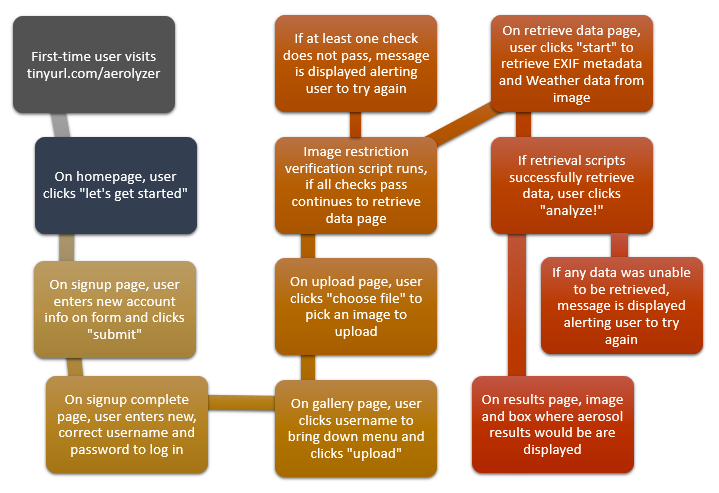
\includegraphics[width=\textwidth]{flow.PNG}
  \caption{Theory of operation flow diagram}
  \label{fig:flow}
\end{figure}
 
\subsection{Setup}
Because Aerolyzer is a mobile webapp, there is no installation; users simple visit our website at tinyurl.com/aerolyzer in any (relatively) current browser either on mobile or desktop. The site has been tested on the most up-to-date versions of Chrome and Firefox on both mobile and desktop.
 
To run Aerolyzer yourself (either locally or in production), use our \texttt{setup.sh} script, which can be found in our GitHub Aerolyzer\_App repository. The script will ask whether you'd like to run the webapp locally or in production. This script has been tested in both Ubuntu and Mac environments.
 
\section{Learning New Technology}
Throughout this project, we utilized a wide variety of resources to learn new technologies and broaden our coding knowledge. As each of us were working with technologies for which we were unfamiliar, we collectively had to learn how to find answers to our questions using the internet and various other resources.
\medskip
Our primary resource was undoubtedly our client, Dr. Kim Whitehall. As a result of her extensive knowledge of the technologies used in our project, she was consistently able to provide us with help in learning these technologies, whether through direct teaching or simply pointing us in the direction of another useful resource.
\medskip
We also made use of a variety of websites to aid in our learning of these technologies, including specific documentation websites for technologies including Haystack, Django, and Apache Solr, as well as online learning communities for programmers like Stack Overflow and TutorialsPoint. A list of the websites utilized throughout our project can be seen below listed in order of helpfulness.
\begin{enumerate}
    \item http://www.stackoverflow.com
    \item http://www.tutorialspoint.com/
    \item http://www.tangowithdjango.com/book/chapters/bootstrap.html
    \item http://mayukhsaha.wordpress.com/2013/05/09/simple-login-and-user-registration-application-using-django/
    \item http://docs.djangoproject.com/en/1.11/
    \item http://django-haystack.readthedocs.io/en/master/
    \item http://lucene.apache.org/solr/
\end{enumerate}
 
\section{What was Learned}
\subsection{Reilly}
\subsubsection{Technical information}
The technical information I learned was probably my biggest takeaway from this senior capstone project. I had not done extensive web development before (beyond simple HTML and CSS), and we ended up creating an entire web framework: hosting the site, designing the UI, testing features, and more. Specific technical knowledge I gained includes web development (HTML, JavaScript, Bootstrap), Python/various available Python packages, Git, working with PostgreSQL  and Apache Solr database, and using the Django framework.
 
Furthermore, our client explained various parts of our project that she completed as a team member and project manager, such as how to create our own Python package, set up an AWS box, and write installation scripts. Although I did not personally implement these aspects of our webapp, I still learned a lot of technical information about them from our client.
 
\subsubsection{Non-technical information}
Through this project, I learned how to collaborate with other software developers from various backgrounds to create, modify, and test the same code on a public site such as GitHub. Our client was extremely helpful in teaching us best practices for version control, code styling, and code reviews as a team. I also learned how to create efficient and well-written documentation with a group, both in-class and from our client - this includes how to write a Software Requirements Specification, a Software Design Specification, and READMEs.
 
Additionally, we used various types of technologies for which there were not always good (or any) documentation. This difficulty made me greatly improve my ability to research, wade through tutorials/blogs, and exhaust my resources. Whether debugging or just trying to figure out where to start, my teammates and I were always able to figure something out, and my confidence in my software development capabilities has improved as a result.
 
Finally, I gained non-technical knowledge regarding several tools for software development. Our client did a great job of introducing us to common software, such as slack, Google Groups, and a GitHub.io team page.
 
\subsubsection{Project work}
I learned the purpose for designing requirements and specifying your project design before you start working. Had we not completed these documents beforehand, we probably would not have taken the time to get together as a team and thoroughly discuss our vision for the project. Though our requirements and design were certainly not perfect from the get-go, we were able to start with a foundation of what we wanted and work from there as our needs changed.
 
Along those lines, I learned that everything does not always go as planned when creating software and that is okay - looking back at our original documents, there were definitely gaps in our planning, and in general we ran into many issues over the course of our project. These experiences only make me more confident that I will know what to think about next time I start a project, as well as be able to push through (as we did this past year) when there appears to be no solution to an issue.
 
\subsubsection{Project management}
As we managed our project, I learned how to work with individual team member's strengths while also trying to improve our weaknesses and allow for gaining more experience in areas where we were not as skilled. I also improved my understanding about time management in terms of a project timeline: completing a task involves giving yourself time to complete all aspects of that task (research, design, implement, debug, integrate, etc.). A final aspect of project management I learned includes the importance of communication. Making sure every team member was on the same page was extremely helpful throughout our project. This information is especially important when multiple people are creating pieces of code that eventually must work together.
 
\subsubsection{Working in teams}
Being on a team consisting of my peers and our client taught me how to work with people of different skill levels. My student team members and I are all about on the same level, though our programming skills differ in specific areas based on our experiences. On the other hand, our client's skills are of course well beyond my own; it was great to learn from her and also learn how to work with someone so advanced in programming/development. My student team members taught me a lot also: I have become better at debugging, working as a team to brainstorm, and collaborate to think through software design from different perspectives.
 
\subsubsection{If you could do it all over, what would you do differently?}
Without considering being able to change the course organization itself, I would have started development earlier than winter term. I also would not have spent so much time worrying about specific details of our documentation. In general, it would have been better to make sure our documents covered all aspects of our project rather than try to have everything figured out on a small scale; we would have benefitted from larger-scale thinking in our design and requirements.
Overall, though, I am really happy with where our project ended up. Our client was great, my team members were great, and my experience overall was positive.
 
\subsection{Sophia}
\subsubsection{Technical information}
This project helped me learn so much more about databases, testing, and web frameworks. Coming into this project, I had not taken databases yet so they were not my strong suit. My goal was to finish this year with a stronger knowledge of databases and I accomplished my goal. One of the things that helped me the most was doing the tech review. This document allowed me to research all of the different types of databases, and learn the pros and cons of each of them. Throughout our project we switched databases, so this allowed me to learn how to use more than one database.
Even though we did not actually implement any tests, I set up TravisCI, Coveralls, and a testing suite. By researching each of these technologies, I have learned a lot more about how to test code which is essential to creating a good project. 
Before this project, I had not used a web framework before. This project has taught me that frameworks are extremely useful and save a lot of time. A great thing about learning Django is that frameworks are pretty similar across the board so learning how to use another framework will be a lot easier.
\subsubsection{Non-technical information}
The non-technical skills that I have gained are documentation, communication, and responsibility. This year I have written more documents than I have in any other class.During the writing process I remember thinking that the work was tedious, but looking back the documentation really helped make the project go smoother. The tech review was a great way to look at all of the available technologies to make sure that we were using the best technology for our problem. I feel like I have grown a lot as a writer and I really appreciate all of the feedback we have gotten from both the professors and the TA's. 
This class has also helped my communication skills. Between practicing our elevator pitches in class, doing a mock poster presentation with another group, and practicing our pitches with our client, I felt really confident and ready for Expo and I had a lot of fun presenting to people. This class has also helped me with time management and responsibility. Setting deadlines for myself was key to doing my work well and in a timely manner.
\subsubsection{Project work}
My biggest takeaway from project work is that a project is not all about the technical part and coding, a successful project requires planning and documentation. We would not have been as successful if we had start coding day one without doing any of the research and planning that we did. We would have been switching around technologies a lot more, and forgetting to do certain requirements.  
\subsubsection{Project management}
A huge part of why our team was so successful is that we played to our strengths and helped cover each other's weaknesses, we delegated every task, and we helped each other. One thing I really liked about this project is that every team member took on tasks that were not our strong suit, but we helped each other through it and that is how to grow as a team and as a software engineer.
\subsubsection{Working in teams}
Through this project I learned that working well in teams helps a person grow so much more than a person working by themselves. Our group did a lot of bonding early fall term and that made a huge difference in our team dynamic the rest of the year. We knew that we could count on each other to do good work, and help one another when we were struggling with some issue. 
\subsubsection{If you could do it all over again, what would you do differently?}
 If I were to do all of this over again I would work harder and think through the documentation. Having a good plan and preparing makes all of the difference when making an application. Our team did really well in planning the project, but we could have thought through our design document more. Good planning can really save a lot of time in the long run.
 
\subsection{Jesse}
\subsubsection{Technical information}
Over the course of this year-long project, I learned a great deal of technical information for which I had no prior experience. Two of my main goals heading into this project were to gain experience in backend development, as well as develop my knowledge of Python programming. Overall, I believe that I accomplished these goals, as I spent the majority of my time working on the backend using Python to handle and process the image data. Through my technical contributions, I would argue that I developed a working knowledge of the Python programming language, as well as gained invaluable experience in backend software development.
 
 
Coming into this project, I also had little to no prior experience with version control. Therefore, one of the greatest pieces of technical knowledge I garnered from this experience was how to use GitHub, as well as the importance of maintaining version control throughout a project.
 
\subsubsection{Non-technical information}
In regards to non-technical information, I learned a great deal about documentation and communication from this project. Through the development of our requirements document, design document, and technology review, my understanding of documentation and its role in project development grew substantially. Moreover, over the course of this year, I also learned a lot about communication and how to work as a team from my team and client.
 
Through our constant collaboration, my teammates helped me to develop my communication skills, and allowed me to contribute significantly to this project. Moreover, I not only learned how to communicate, but I also learned how to collaborate and utilize the ideas of all team members. Finally, through constant interaction with our client, I learned about the importance of communication and honed my ability to communicate effectively over the course of this project.
 
\subsubsection{Project work}
While I have learned a great deal about project work throughout this project, one of the most important takeaways for me has been that project work is not all coding. In fact, most project work, especially in the early stages, focuses on documentation and developing a design plan which the project will reference throughout development. However, I also learned that changes to the documentation and design plan are inevitably going to occur. Therefore, being able to adapt and maintain accurate documentation is of the utmost importance.
 
\subsubsection{Project management}
As far as project management goes, I learned a lot about how to collaboratively delegate work, utilize strengths and weaknesses of various team members, and how to manage time effectively. Throughout our development process, we had several tasks which we delegated out to specific team members in order to efficiently complete work. We also focused on improving our weaknesses while utilizing individual strengths to assist each other throughout the learning process. Through developing collaborative documents and dealing with numerous deadlines, I learned a lot about how to manage time effectively and make sure all team members are on task.
 
\subsubsection{Working in teams}
Through this project, I learned more than I expected to about how to work effectively as a team. Not only does teamwork require great communication, but it requires compromise, substantial effort from each team member, and trust. When working as a team on projects, especially projects that last a long period of time, these factors are essential to keeping a team together and functioning. I believe our weekly client meetings were a driving factor in our team's success. Moreover, our ability to collaborate productively and trust each other with our respective work was essential to our accomplishments.
 
\subsubsection{If you could do it all over again, what would you do differently?}
If I could do this project over again, there are a couple things I would do differently. First of all, I would focus on coming up with creative solutions to the problems given to me by my client, as opposed to simply implementing their recommendations. As a programmer it is easy to just code what you're told to code; however, I believe part of being a programmer is coming up with creative solutions that complete your task as efficiently as possible. This is true especially when working with a client who does not have experience in programming. They may recommend some method for completing the tasks they hand you, when in reality you as a programmer may understand that a different method could be more efficient for solving your problem.
 
Another thing I would do differently is focus on having fun and working with my group to really make the project our own. Coming into capstone I felt relatively intimidated and stressed by the seriousness of the course. However, as I approach completion of the course, I see how the purpose of capstone is truly focused on my development and preparing me for work in the real world. Therefore, I would focus on trying to have fun with this project and explore some creative options that could improve our end product and provide me and my teammates with more knowledge in a different area of programming.
 
\section{Appendix 1: Essential Code Listing} \label{appendix}
The following code is the core of our webapp framework. Each webpage is constructed as a "view" in Django, shown in \texttt{views.py} below. Functionality for phase 2 is included as comments/pseudocode.
\begin{lstlisting}[language=python]
from django.http import HttpResponse
from django.shortcuts import render
from app.forms import *
from aerolyzer import *
from django.contrib.auth.decorators import login_required
from django.contrib.auth import logout
from django.views.decorators.csrf import csrf_protect
from django.http import HttpResponseRedirect
from django.template import RequestContext
from django.contrib.auth import authenticate
from django.contrib.auth.models import User
from django.contrib.auth import authenticate, login
from django.contrib import messages
from django.conf import settings
from django.core.files.storage import FileSystemStorage
from shutil import copyfile
import os
import pysolr
import time
 
 
def index(request):
    if request.method == 'POST':
        usr = request.POST['username']
        psswd = request.POST['password']
        user = authenticate(username=usr, password=psswd)
        if user is not None:
            login(request, user)
            return HttpResponseRedirect('gallery')
        else:
            return render(request, 'app/index.html', {'login_message' :
                'That username/password doesn\'t work!'},)
    return render(request, 'app/index.html', {'user': request.user,
        'is_index':True},)
 
def about(request):
    return render(request, 'app/about.html', {'user': request.user},)
 
def faq(request):
    return render(request, 'app/faq.html', {'user': request.user},)
 
def signup(request):
    if request.method == 'POST':
        form = RegistrationForm(request.POST)
        if form.is_valid():
            user = User.objects.create_user(
            username=form.cleaned_data['username'],
            email=form.cleaned_data['email'],
            password=form.cleaned_data['password1']
            )
            return HttpResponseRedirect('signup_complete')
    else:
        form = RegistrationForm()
    return render(request,
    'app/signup.html',
    {'form': form, 'user': request.user, 'is_index':True,},
    )
 
def signup_complete(request):
    return render(request, 'app/signup_complete.html',{ 'user': request.user },)
 
@login_required
def gallery(request):
    return render(request,
    'app/gallery.html',
    { 'user': request.user },
    )
 
@login_required
def upload(request):
    if request.method == 'POST' and request.FILES['myfile']:
        myfile = request.FILES['myfile']
        fs = FileSystemStorage()
        filename = fs.save(myfile.name, myfile)
        uploadedFileUrl = fs.url(filename)
        request.session['filename'] = filename
        request.session['uploadedFileUrl'] = uploadedFileUrl
        verified = check_image("media/" + filename)
        if not verified['meetsRest']:
            os.remove("media/" + filename)
            return render(request,
            'app/upload.html',
            { 'user': request.user, 'filename': filename, 'uploadedFileUrl': uploadedFileUrl,
            'error_message': verified['error_message'],},)
        else:
            locExifData = verified["locExifData"]
            exifData = verified["exifData"]
            latitude = locExifData['gps gpslatitude']
            d = float(latitude.values[0].num) / float(latitude.values[0].den)
            m = float(latitude.values[1].num) / float(latitude.values[1].den)
            s = float(latitude.values[2].num) / float(latitude.values[2].den)
            exifLat = d + (m / 60.0) + (s / 3600.0)
            if locExifData["gps gpslatituderef"].values[0] != "N":
                exifLat = 0 - exifLat
            longitude = locExifData["gps gpslongitude"]
            d = float(longitude.values[0].num) / float(longitude.values[0].den)
            m = float(longitude.values[1].num) / float(longitude.values[1].den)
            s = float(longitude.values[2].num) / float(longitude.values[2].den)
            exifLong = d + (m / 60.0) + (s / 3600.0)
            if locExifData["gps gpslongituderef"].values[0] != "E":
                exifLong = 0 - exifLong
            location = "%f,%f" % (exifLat, exifLong)
            exifData['location'] = location
            request.session['exifData'] = exifData
            return HttpResponseRedirect('retrieve')
    return render(request, 'app/upload.html', { 'user': request.user, },)
 
@login_required
def profile(request):
    return render(request,
    'app/profile.html',
    { 'user': request.user, },
    )
 
@login_required
def retrieve(request):
    uploadedFileUrl = request.session['uploadedFileUrl']
    filename = request.session['filename']
    exifData = request.session['exifData']
    location = exifData['location']
    if request.method == 'POST':
        weatherData = wunderData.get_data(location)
        if weatherData is None:
            os.remove("media/" + filename)
            return render(request,
             'app/retrieve.html',
            { 'user': request.user, 'exifData' : exifData, 'all_clear': False,
            'error_message': 'weather', 'filename': filename,
            'uploadedFileUrl': uploadedFileUrl,},)
        request.session['wunderData'] = weatherData
        # misrData = retrieve_misr_info(location)
        # if misrData is None:
        #   os.remove("media/" + filename)
        #   return render(request,
        #     'app/retrieve.html',
        #   { 'user': request.user, 'error_message': 'satellite' },
        #     )
        # request.session['misrData'] = misrData
        # return render(request,
        # 'app/retrieve.html',
        # { 'user': request.user, 'exifData' : exifData,
        # 'wunderData': wunderData, 'misrData': misrData, 'all_clear': True, },
        # )
        return render(request,
        'app/retrieve.html',
        { 'user': request.user, 'exifData' : exifData,
        'wunderData': weatherData, 'misrData': 'misr here', 'all_clear': True,
        'filename': filename, 'uploadedFileUrl': uploadedFileUrl,},
        )
 
    return render(request,
    'app/retrieve.html',
    { 'user': request.user, 'filename': filename, 'uploadedFileUrl': uploadedFileUrl,
    'all_clear': False,},
    )
 
@login_required
def results(request):
    uploadedFileUrl = request.session['uploadedFileUrl']
    filename = request.session['filename']
    exifData = request.session['exifData']
    weatherData = request.session['wunderData']
    # misrData = request.session['misrData']
    # aerosol = coreAlgorithmHere(exifData, wunderData, misrData)
    username = request.user.username
    unique = str(int(time.time()))
    solrFilename = username + "-" + unique + "_" + filename
    solr = pysolr.Solr('http://localhost:8983/solr/aerolyzer', timeout=10)
    solr.add([
        {
            "filename": solrFilename,
            "exif": exifData,
            #"misr": misrData,
            "wunder": weatherData,
            #"results": aerosol,
            "username": username,
        },
    ])
    newFilename = os.path.abspath('../..') + "/installDir/" + unique + "_" + filename
    copyfile(os.getcwd() + "/media/" + filename, newFilename)
     # return render(request,
    # 'app/results.html',
    # { 'user': request.user, 'aerosol': aerosol,
    # 'image': retrievedSolrImg},
    # )
    return render(request,
    'app/results.html',
    { 'user': request.user, 'filename': filename, 'uploadedFileUrl': uploadedFileUrl,},)
 
def logout_page(request):
    logout(request)
    return HttpResponseRedirect('/app')
\end{lstlisting}
 
 
\end{flushleft}
\end{document}
 
 
